\chapter{Requirements}

In this chapter, the framework conditions, that exist at Kubermatic and are relevant for the development of the application, are examined.
Following this, requirements for the service that is to be developed are to be derived from the results of the analysis.

\section{Kubermatic Kubernetes Platform}
``Kubermatic Kubernetes Platform (KKP) is in an open source project to centrally manage the global automation of thousands of Kubernetes clusters across multicloud, on-prem and edge with unparalleled density and resilience``~\cite{KKP-GITHUB}.

Due to the need of a central management solution for a multi cluster Kubernetes environment, KKP set foot to solve this problem.
It aims to give the customer everything needed to build their own Kubernetes cloud environment. 
This includes a Multicloud Self Service Portal, HA Self-healing Infrastructure, Multi-tenancy and User Management, Monitoring and more.
A detailed list of the key features can be found on the Kubermatic website.\footnote{https://www.kubermatic.com/products/kubermatic/}
\\
To achieve resilience, KKP relies on Kubernetes itself.
This requires a so-called master cluster in which Kubermatic is installed, the master is the central instance in which all clusters are managed via KKP API.

\begin{figure}[H]
    \centering
    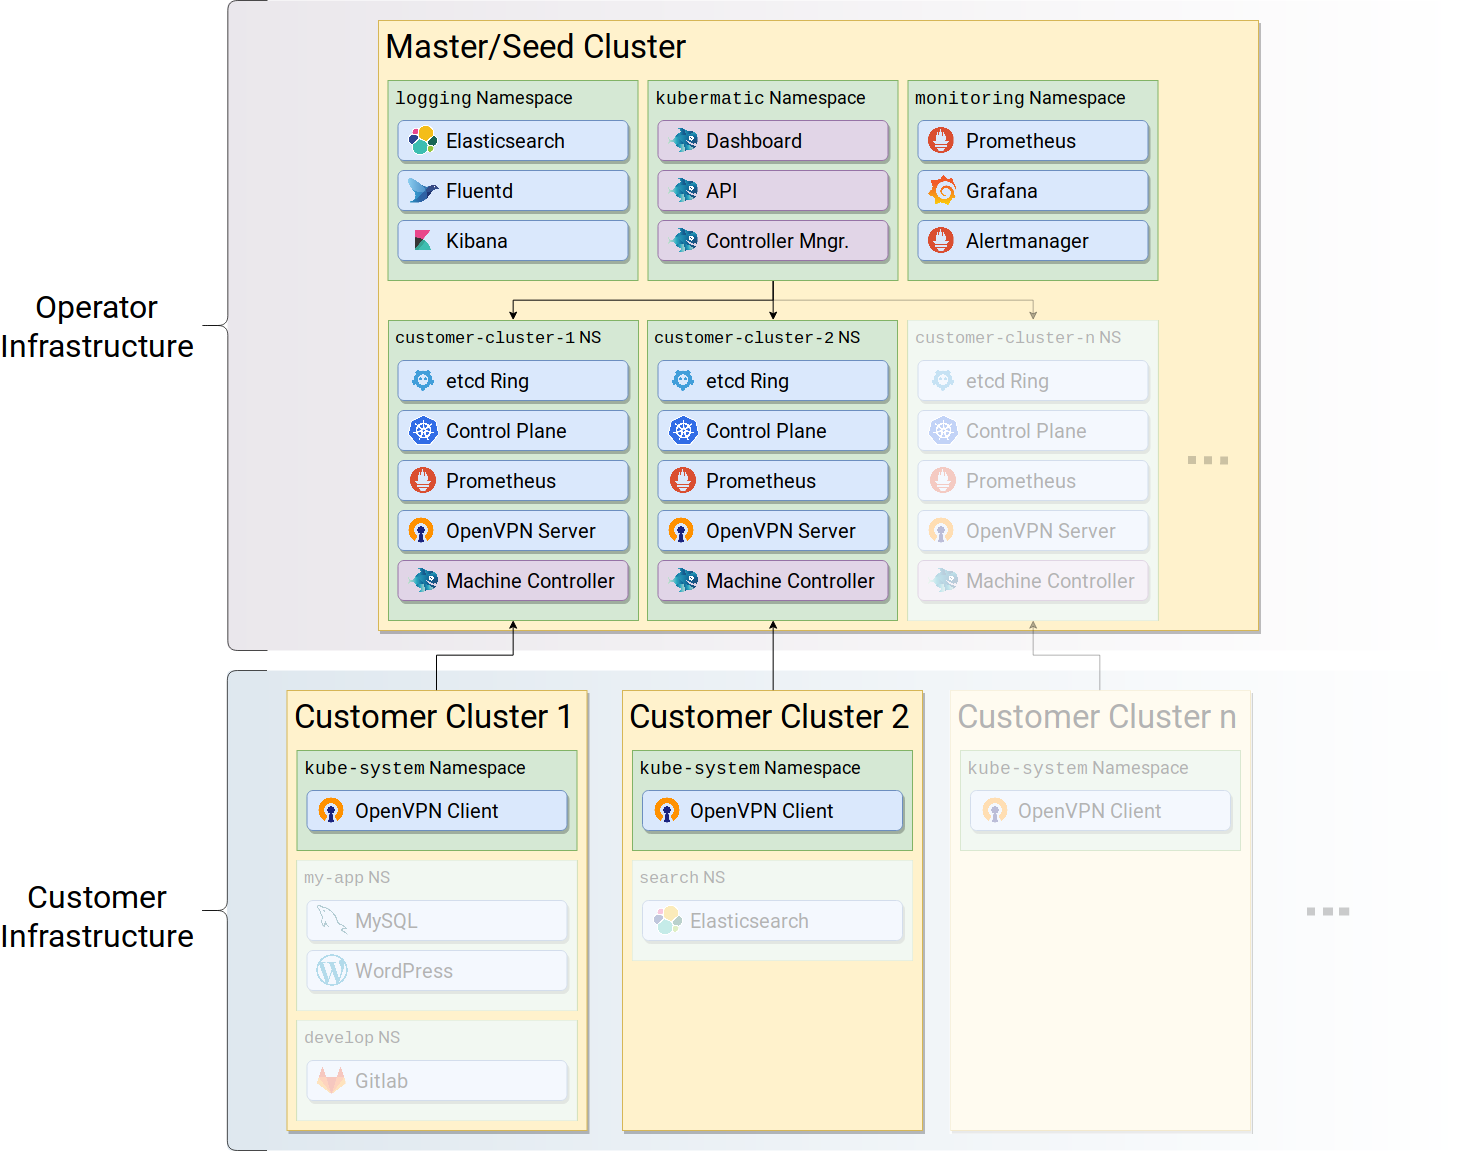
\includegraphics[width=1\textwidth, left]{media/05/kkp}
    \caption{"Kubermatic architecture, combined master seed" by Kubermatic GmbH CC BY 4.0}
    \label{fig:kubermatic}
\end{figure}

Another concept is the seed cluster, in which among other parts, the control-plane of a kubernetes cluster, that was created via KKP, lives.
As \autoref{fig:kubermatic} shows, the seed cluster can be the same as the master, but it is not mandatory.
Especially for large scale deployments it is recommended to run several independent seed clusters.
Thus, only worker nodes have to be created and connected.
Virtual machines are created via a supported provider, which are then provisioned by KKP and added as nodes.
\\
The master as well as the seed cluster should be operated in a high availability setup.
This offers the advantage that the Kubernetes control plane of the customer cluster is automatically a High Availability setup.


\section{KubeLB}\label{sec:KubeLB}

The idea behind KubeLB is to adopt concepts of KKP for load balancing in multicloud, on-prem and edge Kubernetes environments.
As mentioned in \autoref{sec:ExternalLoadBalancer}, load balancers need to be integrated manually to every cluster.
This is especially needed for bare metal environments, where no cloud provider solution is available.
The already existing open source solutions for the implementation of the load balancer target single Kubernetes clusters and are not designed for a highly dynamic multi cloud infrastructure.
\\
The main feature is the easy integration and availability of load balancing in many, dynamically created, Kubernetes clusters.
These clusters are referred to as \textit{user clusters} in the following.
For this purpose, a dedicated cluster is provided, which deploys a load balancer within the cluster, referred to as \textit{load balancer cluster} in the following.
In order to expose the load balancer in the cluster to the outside world, it is necessary for the load balancer cluster to have a load balancer implementation.
This has the advantage that load balancer integration only has to be performed once for the load balancer cluster, and simplifies the management of external IP addresses, as these can be managed centrally.
All features of the Kubernetes Service object of the load balancer type should be supported.
\\
In addition to the load balancer integration, layer 7 load balancing should also be offered.
This refers in particular to the Ingress resource and the ingress controller.
Since this, like the load balancer, is not automatically available within a Kubernetes cluster, integration should also be offered here.
For this purpose, a load balancer with Layer 7 properties, analogous to the Layer 4 load balancer, is to be deployed and made available within the load balancer cluster.
All features of the Kubernetes ingress object should be supported.
\\
To pass the requests for a load balancer or an ingress resource to the load balancer cluster, an agent is provided within the user clusters.
The agent acts as a kind of cloud controller\footnote{https://kubernetes.io/docs/concepts/architecture/cloud-controller/}, which manages external resources of the cluster.
\\
It is common within the cloud native community to create a proposal alongside contributions.
A proposal should describe what the idea is, the goals that are being pursued, and include an architectural overview.
The original proposal for KubeLB can be found in the Kubermatic repository\footnote{https://github.com/kubermatic/kubermatic/blob/master/docs/proposals/kubelb.md} on GitHub.
